\documentclass[aspectratio=169]{beamer}
\usepackage{amsmath, amssymb}
\usepackage{graphicx}
\usepackage{xcolor}
\usepackage{tikz}
\usetikzlibrary{arrows.meta}
\usetikzlibrary{positioning}
\usetikzlibrary{shapes.geometric}
\tikzset{
    sommet/.style = {circle, draw, on grid},
    c1/.style = {fill=orange!50},
    c2/.style = {fill=teal!50},
    c3/.style = {fill=violet!50},
    >=Latex
}
\usepackage[boxed]{algorithm2e}
\SetKwProg{Algo}{algorithm}{}{}
\usepackage{appendixnumberbeamer}
\everymath{\displaystyle}

% Metropolis theme
\usetheme{metropolis}
\usefonttheme[onlymath]{serif}
\metroset{progressbar=frametitle}
\metroset{titleformat=smallcaps}
\metroset{numbering=fraction}
\metroset{block=fill}
\definecolor{mypink}{HTML}{e91e63}
\setbeamercolor{alerted text}{fg=mypink}

\makeatletter
\setlength{\metropolis@titleseparator@linewidth}{1pt}
\setlength{\metropolis@progressonsectionpage@linewidth}{1.5pt}
\setlength{\metropolis@progressinheadfoot@linewidth}{2.5pt}
\makeatother

\title{Combinatorial Auctions with Restricted Complements}
\subtitle{An article by I. Abraham, M. Babaioff, S. Dughmi and T. Roughgarden}
\author{Hugo \textsc{Boulier}, Hugo \textsc{Francon} \& Igor \textsc{Martayan}}
\date{November 8, 2021}

\begin{document}

{\metroset{background=dark}\maketitle}

\begin{frame}{Introduction}
    \begin{columns}
        \column{0.6\textwidth}
        \begin{itemize}
            \item Auction with $n$ bidders and $m$ items
            \item Some item groups gain added value when purchased together
            \item Use of hyperedges to model these preferences
        \end{itemize}

        \column{0.4\textwidth}
        \begin{figure}
            \centering
            \begin{tikzpicture}[node distance=0.25cm and 0.25cm]
                \node (complet) [inner sep=1pt] {\small 10};
                \node (galette) [label={\scriptsize 0.5}, above left=of complet] {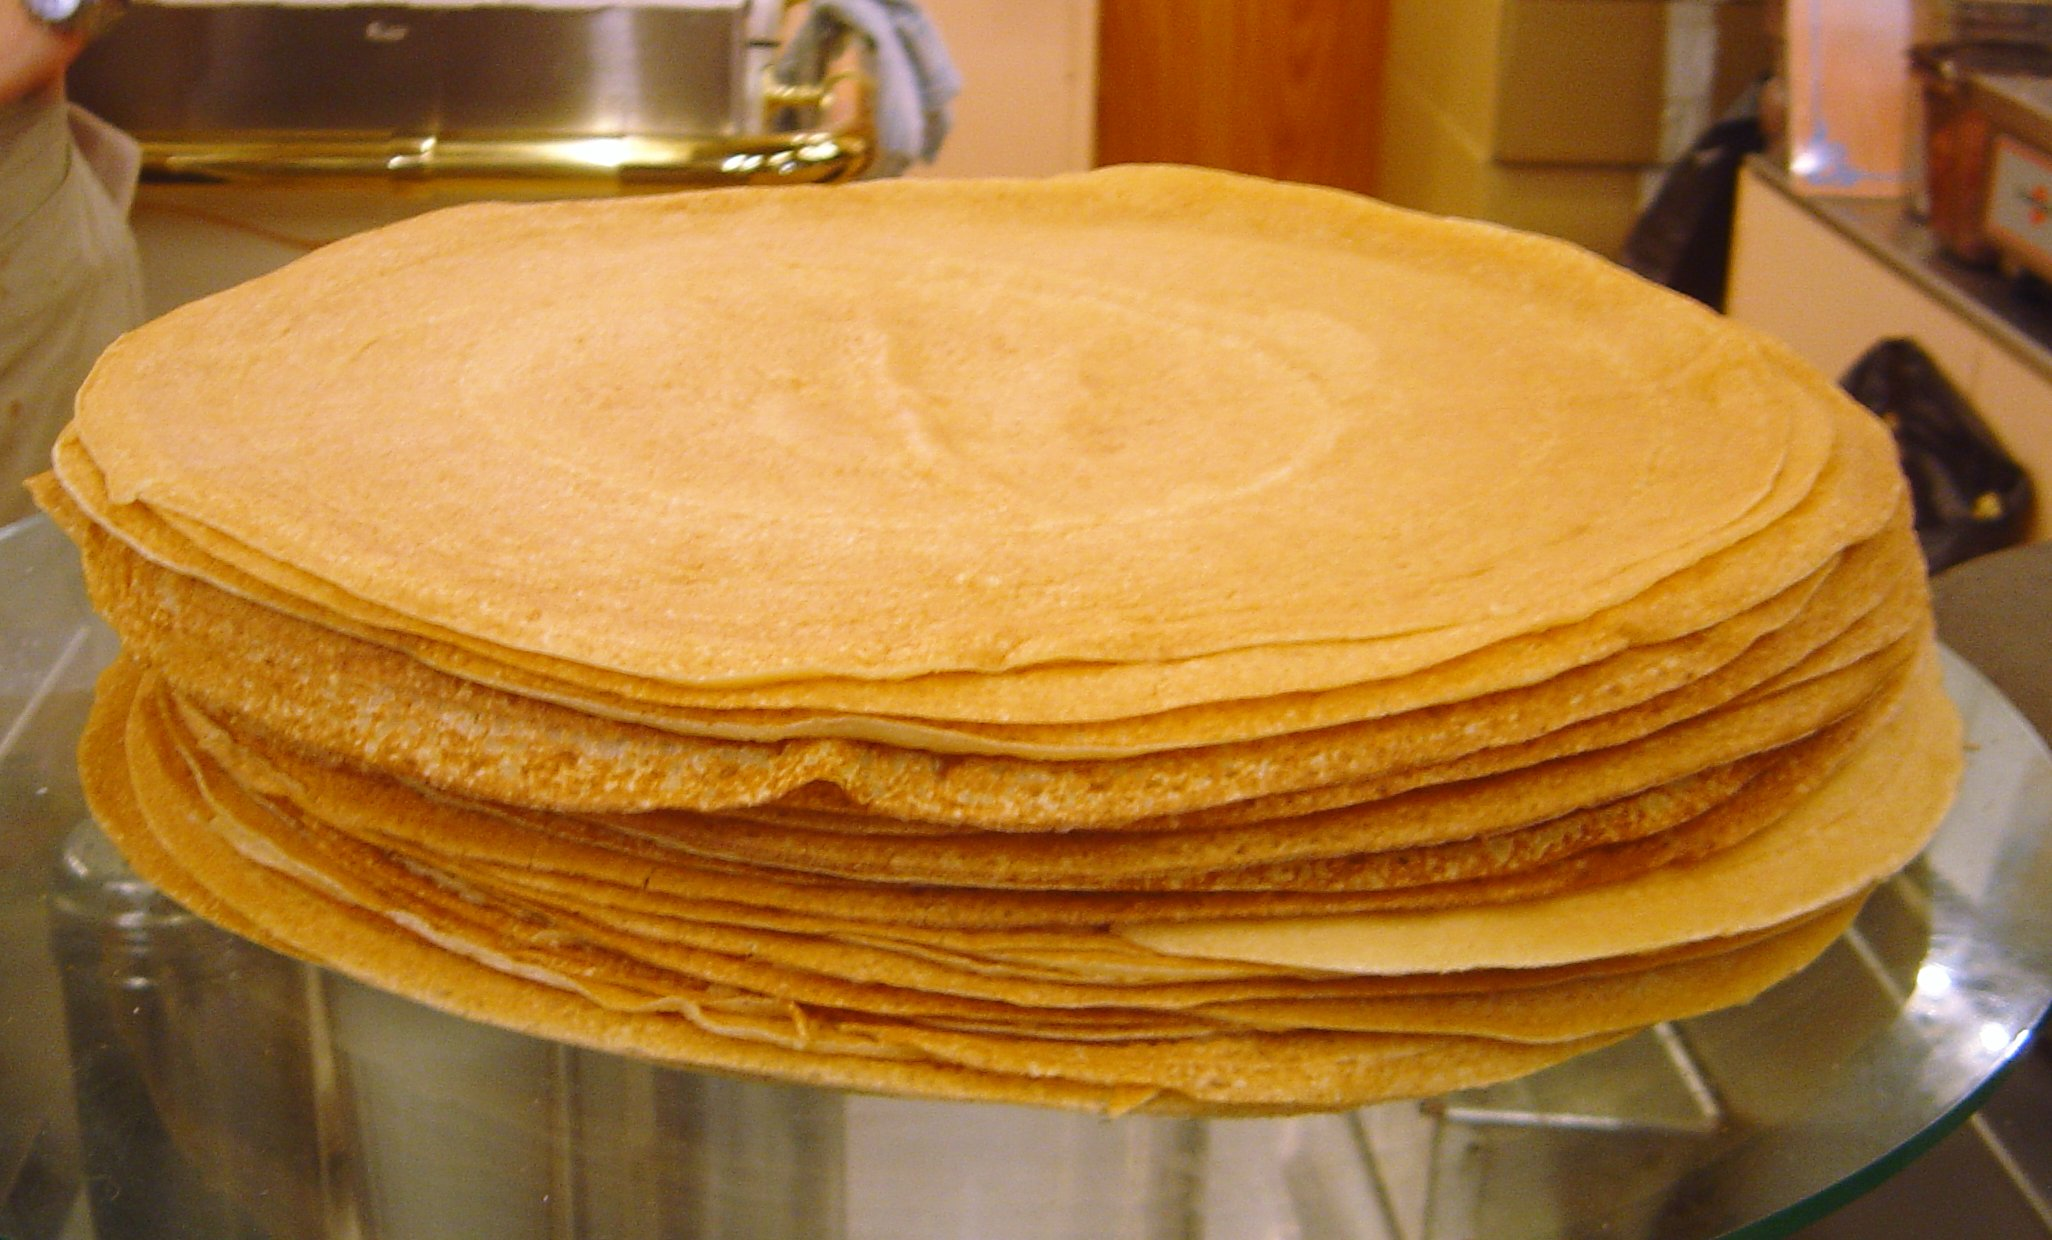
\includegraphics[width=0.4\textwidth]{img/crepe.jpg}};
                \node (oeuf) [label={\scriptsize 2.5}, above right=of complet] {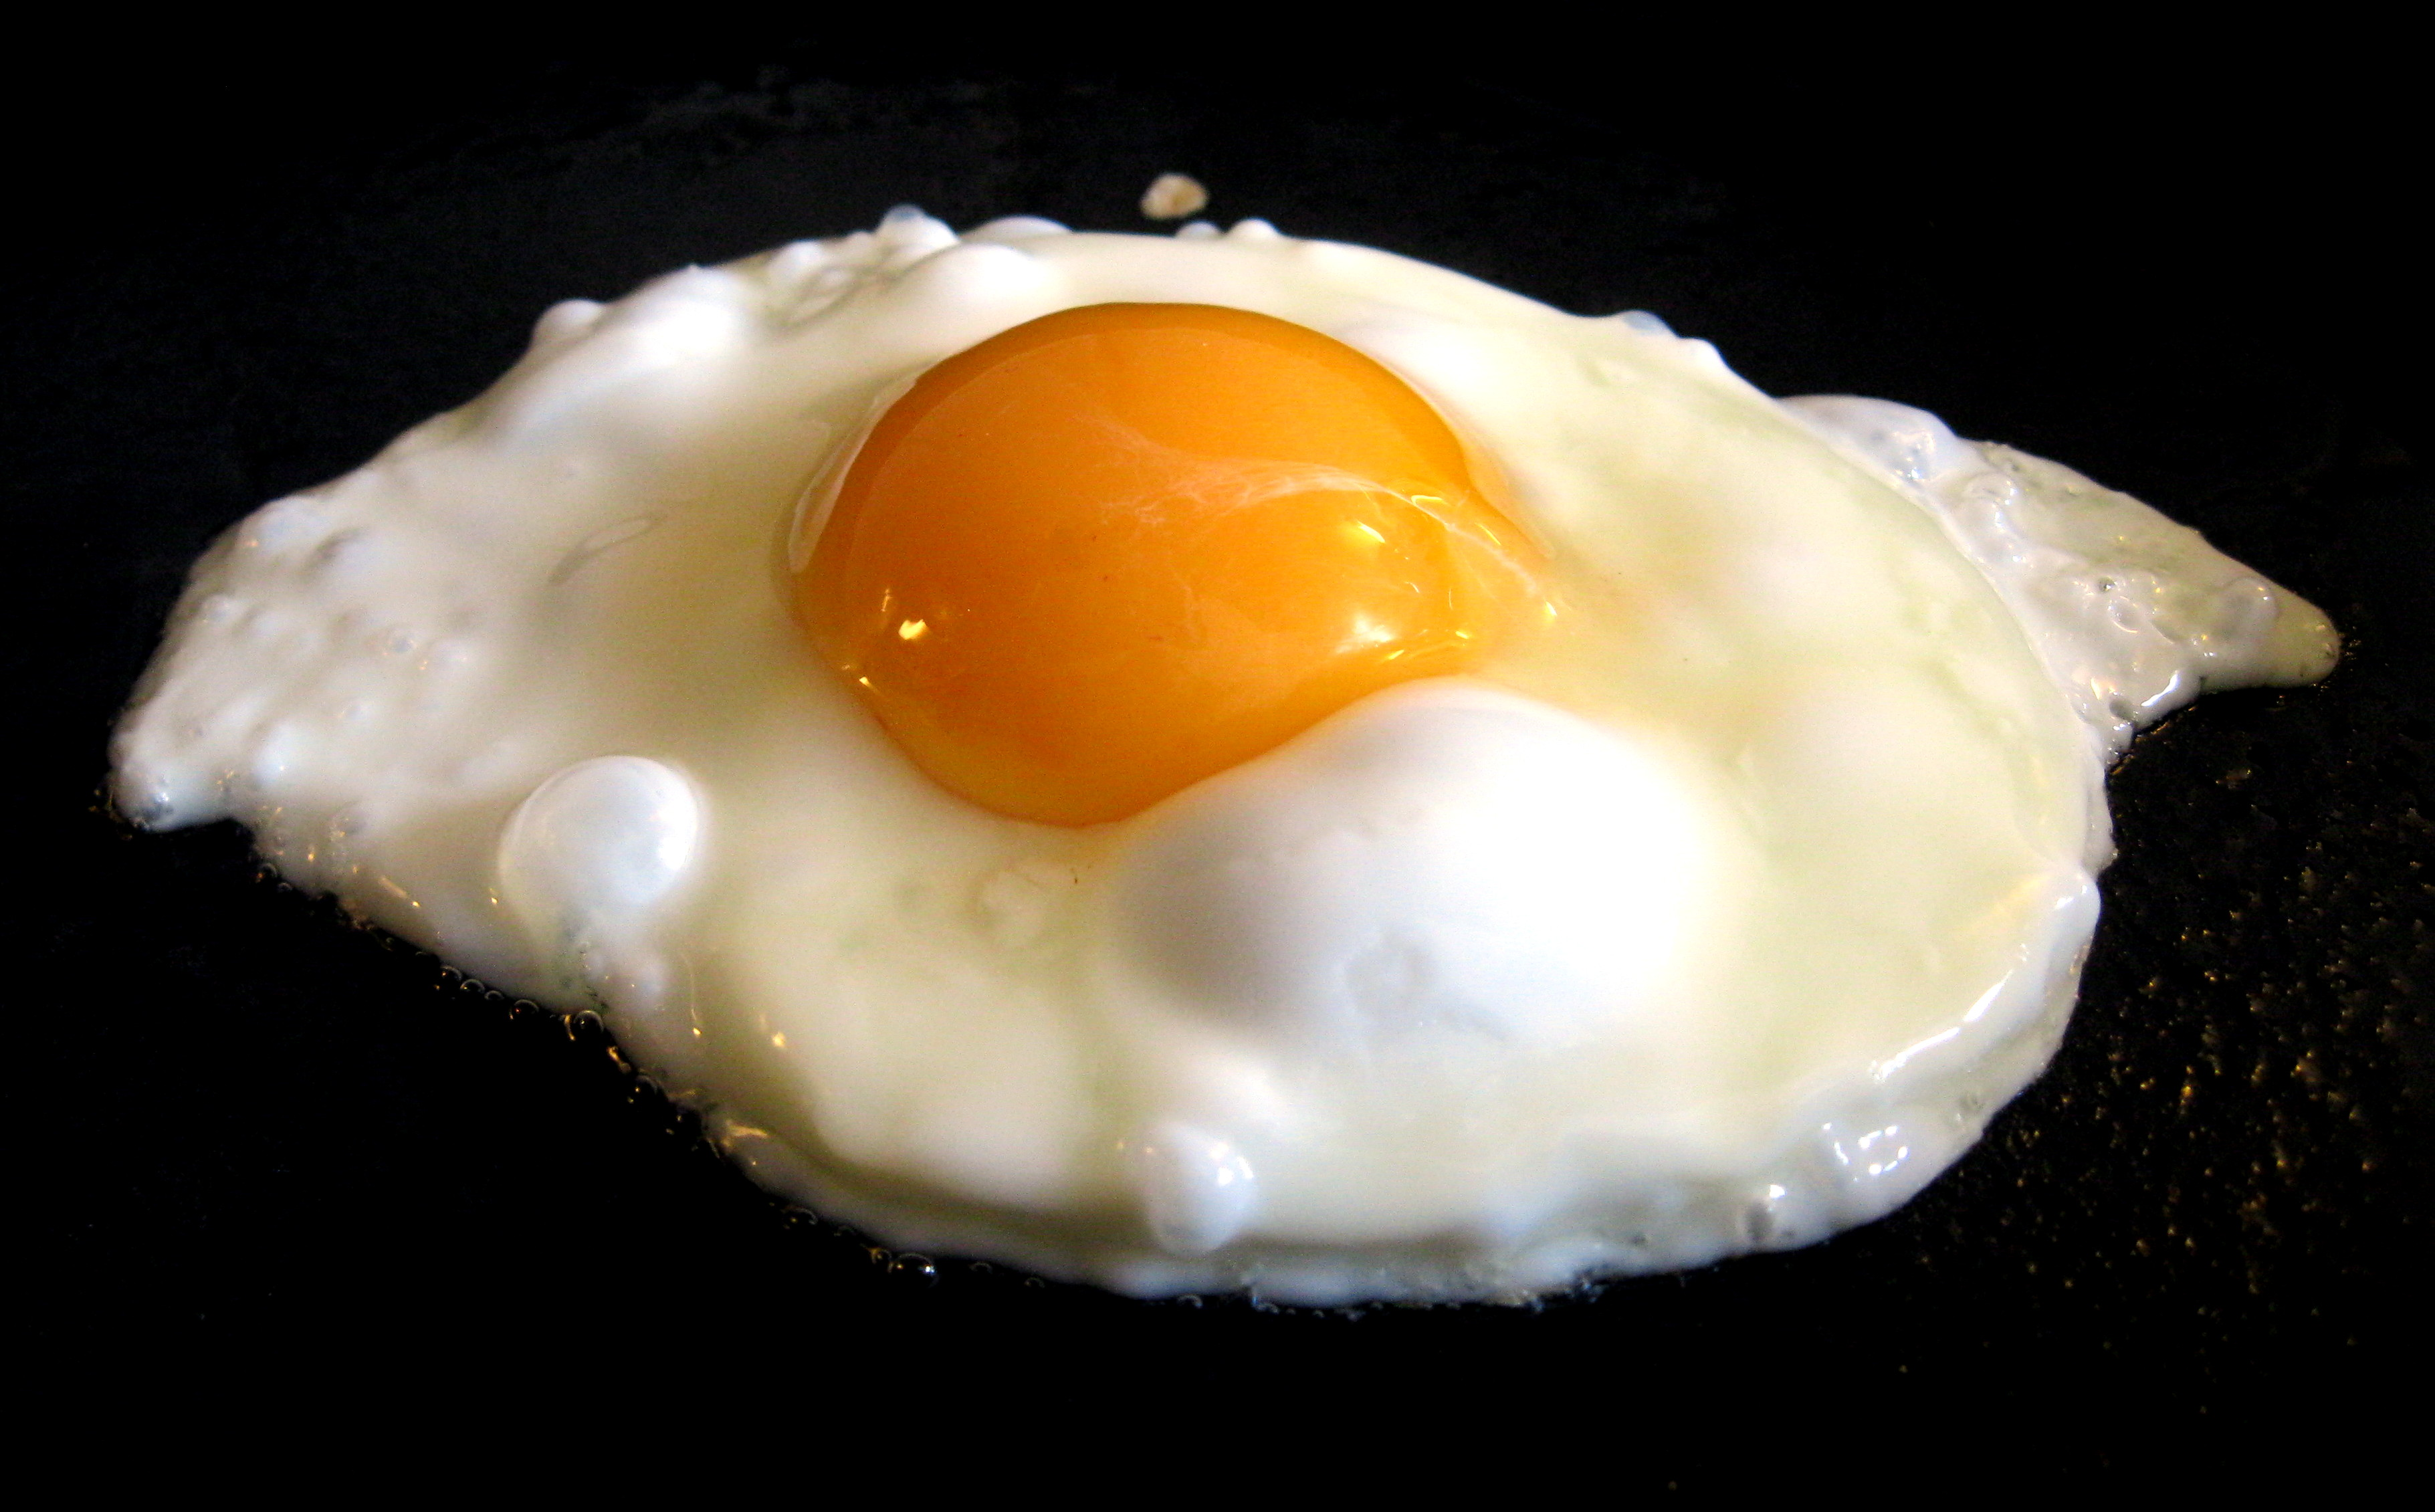
\includegraphics[width=0.4\textwidth]{img/oeuf.jpg}};
                \node (jambon) [label={\scriptsize 1.5}, below left=of complet] {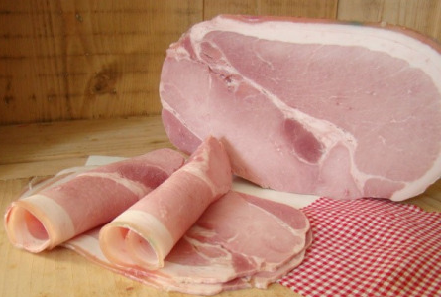
\includegraphics[width=0.4\textwidth]{img/jambon.png}};
                \node (fromage) [label={\scriptsize 2.5}, below right=of complet] {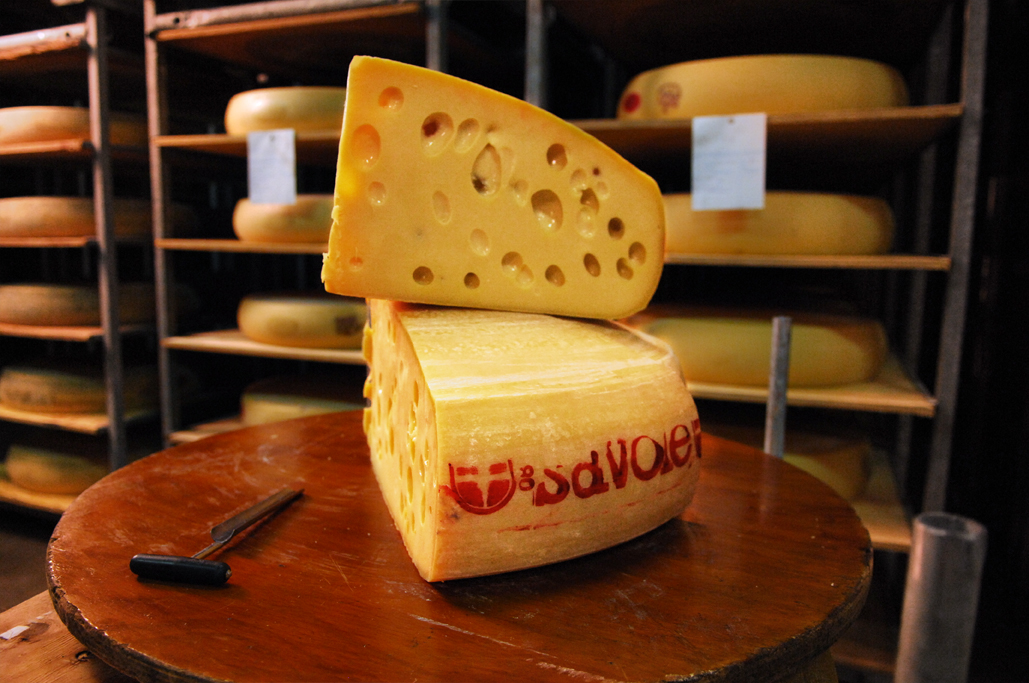
\includegraphics[width=0.4\textwidth]{img/fromage.jpg}};
                \draw (galette) -- (complet) -- (jambon) -- (complet) -- (oeuf) -- (complet) -- (fromage);
            \end{tikzpicture}
        \end{figure}
    \end{columns}
\end{frame}

\begin{frame}{Core Questions}
    \begin{enumerate}
        \item Polynomial approximation for \alert{planar graphs}?
        \item Polynomial approximation for \alert{hypergraphs}?
        \item \alert{Truthful version} of this approximation?
    \end{enumerate}
\end{frame}

{\metroset{background=dark}\section{Polynomial approximation for planar graphs}}

\begin{frame}{Baker's technique for polynomial approximation}
    \begin{columns}
        \column{0.6\textwidth}
        \begin{block}{Baker's decomposition [Baker, 1994]}
            A \alert{planar graph} $G$ can be partitioned into $P_0, \dots, P_k$ such that for each $i$, $G \setminus P_i$ has a \alert{treewidth} $\leqslant 3k$.
        \end{block}

        $\hookrightarrow$ very useful for \alert{polynomial approximations}

        \begin{block}{Generalization with minors [DeVos, 2004]}
            The same method can be applied for any graph that \alert{excludes a given minor} $X$.
        \end{block}

        \column{0.4\textwidth}
        \begin{figure}
            \centering
            \begin{tikzpicture}
                \node (0A) at (0, 1) {};
                \node (1A) [sommet, c1] at (0,0) {};
                \path[->] (0A) edge (1A);
                \node (2A) [sommet, c2] at (-1, 0) {};
                \node (2B) [sommet, c2] at (0, -1) {};
                \node (2C) [sommet, c2] at (1, 0) {};
                \path (1A) edge (2A) edge (2B) edge (2C);
                \node (3A) [sommet, c3] at (-1, -1) {};
                \node (3B) [sommet, c3] at (0, -2) {};
                \node (3C) [sommet, c3] at (1, -2) {};
                \node (3D) [sommet, c3] at (2, -1) {};
                \path (2B) edge (2A) edge (2C) edge (3A) edge (3B) edge (3C)
                (2C) edge (3C) edge (3D);
                \node (4A) [sommet, c1] at (-1, -2) {};
                \node (4B) [sommet, c1] at (0, -3) {};
                \node (4C) [sommet, c1] at (1, -3) {};
                \node (4D) [sommet, c1] at (2, -3) {};
                \node (4E) [sommet, c1] at (3, -2) {};
                \path (3A) edge (4A) edge (4B)
                (3B) edge (3C) edge (4B) edge (4C)
                (3C) edge (3D) edge (4C) edge (4D) edge (4E)
                (3D) edge (4E);
                \node (5A) [sommet, c2] at (0, -4) {};
                \node (5B) [sommet, c2] at (1, -4) {};
                \node (5C) [sommet, c2] at (2, -4) {};
                \path (4A) edge (4B) edge (5A)
                (4B) edge (4C) edge (5A) edge (5B)
                (4C) edge (5B)
                (4E) edge (4D) edge (5C)
                (5B) edge (5C);
            \end{tikzpicture}
        \end{figure}
    \end{columns}
\end{frame}

\begin{frame}{Polynomial-time approximation for planar graphs}
    \begin{block}{Algorithm}
        \begin{enumerate}
            \item \alert{Partition} $G$ into $P_0, \dots, P_k$ such that each $G_i = G \setminus P_i$ has a \alert{fixed treewidth}
            \item Compute the \alert{tree decomposition} of each $G_i$
            \item Compute the optimal allocation $A_i$ for each tree with \alert{dynamic programming}
            \item Return $A^* = \arg \max_{A_i} \sum_{j \in N} v_j(A_i^{-1}(j))$
        \end{enumerate}
    \end{block}

    $\hookrightarrow$ polynomial $(1 + \varepsilon)$-approximation

    \begin{block}{Truthfulness}
        Once combined with \alert{VCG payment}, this mechanism is \alert{truthful}.
    \end{block}
\end{frame}

\begin{frame}[standout]
    Can we generalize this approach for \alert{hypergraphs}?
\end{frame}

\begin{frame}{Approximate welfare maximization algorithm}
    \begin{columns}
        \column{0.6\textwidth}
        We generalize to \(r\)-hypergraph with \alert{nonnegative hyperedge weight}

        \begin{block}{Polynomial time \(r\)-approximation}
            The welfare maximization problem can be \(r\)-approximated in polynomial time.
        \end{block}

        \begin{block}{Known lower bound [Trevisan, 2001]}
            There is no \(r/2^{O(\sqrt{\log r})}\)-approximation.
        \end{block}

        \column{0.4\textwidth}
        2 step algorithm:
        \begin{itemize}
            \item (real) linear programming
            \item randomized assignment
        \end{itemize}
    \end{columns}
\end{frame}

\begin{frame}{The linear program}
    \[
        \text{maximize:} \sum_{i \,\in \{\text{bidders}\}} \left(
        \sum_{j \,\in \{\text{items}\}} w_{ij}\, {\color{orange} x_{ij}}
        + \sum_{e \,\in \{\text{edges}\}_i} w_{ie}\, {\color{blue} z_{ie}}
        \right)
    \]
    with
    \begin{align*}
        \sum_{i \,\in \{\text{bidders}\}} {\color{orange} x_{ij}}  = 1 & \hspace{.5cm} \text{for all item \(j\)}                              \\
        {\color{blue} z_{ie}}  \leqslant {\color{orange} x_{ij}}       & \hspace{.5cm} \text{for all player \(i\), edge \(e\) and item \(j\)} \\
        {\color{orange} x_{ij}}   \geqslant 0                          & \hspace{.5cm} \text{for all player \(i\) and item \(j\)}             \\
        {\color{blue} z_{ie}}  \geqslant 0                             & \hspace{.5cm} \text{for all player \(i\) and edge \(e\)}
    \end{align*}

    $\hookrightarrow$ Real-valued valuation in \alert{polynomial time}.
\end{frame}

\begin{frame}{The randomized rounding algorithm}
    \begin{columns}
        \column{0.65\textwidth}
        \hrule
        \vspace{.1cm}
        \textbf{Input:} an optimal (real) solution \((x^*, z^*)\) of the linear program

        \vspace{.65cm}
        \textbf{While} there exists an unassigned item
        \begin{enumerate}
            \item choose a player \(i\) at random
            \item choose a threshold \(t \in [0, 1]\) at random
            \item assign to \(i\) every unassigned item with \(x_{ij}^* \geqslant t\)
        \end{enumerate}
        \hrule

        \column{0.35\textwidth}
        Probability that player \(i\) gets edge \(e\) greater than \(\frac{z_{ie}^*}{|e|} \geqslant \frac{z_{ie}^*}{r}\)

        \(\hookrightarrow\) \(r\)-approximation

    \end{columns}
    \pause
    \begin{center}
        \alert<2>{Not Truthful}
    \end{center}
\end{frame}

\begin{frame}[standout]
    Can we find a \alert{truthful version} of this approach?
\end{frame}

\begin{frame}{A truthful approximation mechanism}
    \begin{columns}
        \column{0.6\textwidth}
        ...

        \column{0.4\textwidth}
        ...
    \end{columns}
\end{frame}

\begin{frame}{Conclusion}
    ...
\end{frame}

\appendix

{\metroset{background=dark}\section{Appendix}}

\begin{frame}{Planar graphs characterization with minors}
    \begin{columns}
        \column{0.6\textwidth}
        \begin{block}{Kuratowski's theorem}
            A graph is planar if and only if it does not contain \textcolor{violet}{$K_5$} or \textcolor{teal}{$K_{3,3}$} as a minor.
        \end{block}

        \column{0.4\textwidth}
        \begin{figure}
            \centering
            \begin{tikzpicture}
                \node[regular polygon, regular polygon sides=5, minimum size=2cm] (P) {};
                \foreach \i in {1, ..., 5} {
                        \node (\i) [sommet, c3] at (P.corner \i) {};
                    }
                \foreach \i in {1, ..., 5} {
                        \foreach \j in {\i, ..., 5} {
                                \draw (\i) -- (\j);
                            }
                    }
            \end{tikzpicture}
        \end{figure}
        \begin{figure}
            \centering
            \begin{tikzpicture}[node distance=1cm and 1cm]
                \node (A) [sommet, c2] {};
                \node (B) [sommet, c2, right=of A] {};
                \node (C) [sommet, c2, right=of B] {};
                \node (D) [sommet, c2, below=of A] {};
                \node (E) [sommet, c2, right=of D] {};
                \node (F) [sommet, c2, right=of E] {};
                \path (A) edge (D) edge (E) edge (F)
                (B) edge (D) edge (E) edge (F)
                (C) edge (D) edge (E) edge (F);
            \end{tikzpicture}
        \end{figure}
    \end{columns}
\end{frame}

\end{document}
